\documentclass[10pt,a4paper]{ltjsarticle}       % LuaTeX を使う
\usepackage[luatex]{graphicx}             % LuaTeX 用, draft がついているときは図の代わりに同じ大きさの枠ができる
\usepackage{here}                               % 図表の位置を強制して出力
\usepackage{afterpage}                          % 残っている図を貼り付ける(\afterpage{\clearpage})
\usepackage[subrefformat=parens]{subcaption}    % サブキャプション(図1(a) とか)
\usepackage{setspace}                           % 行間制御
\usepackage{ulem}                               % 下線や取り消し線など
\usepackage{booktabs}                           % きれいな表(\toprule \midrule \bottomrule)
\usepackage{multirow}                           % 表で行結合
\usepackage{multicol}                           % 表で列結合
\usepackage{hhline}                             % 表で 2 重線
\usepackage[table]{xcolor}                      % カラー
\usepackage{tikz}                               % 図描画用
\usepackage[framemethod=tikz]{mdframed}         % 文章を囲むとき用
\usepackage[version=3]{mhchem}                  % 化学式
\usepackage{siunitx}                            % 単位
\usepackage{comment}                            % コメント
\setcounter{tocdepth}{3}                        % 目次に subsubsection まで表示
\usepackage{listings}
\lstdefinelanguage{Julia}%
  {morekeywords={abstract,break,case,catch,const,continue,do,else,elseif,%
      end,export,false,for,function,immutable,import,importall,if,in,%
      macro,module,otherwise,quote,return,switch,true,try,type,typealias,%
      using,while},%
   sensitive=true,%
   alsoother={\$},%
   morecomment=[l]\#,%
   morecomment=[n]{\#=}{=\#},%
   morestring=[s]{"}{"},%
   morestring=[m]{'}{'},%
}[keywords,comments,strings]%

\lstset{%
    language         = Julia,
    basicstyle       = \ttfamily,
    keywordstyle     = \bfseries\color{blue},
    stringstyle      = \color{magenta},
    commentstyle     = \color{ForestGreen},
    showstringspaces = false,
}
%\lstset{
%    frame=single,
%    basicstyle=\small\ttfamily,
%    tabsize=4,
%    language=python,
%    keywordstyle=\color{red},
%    stringstyle=\color{blue}
%}

% -----ヘッダ・フッタの設定-----
\usepackage{fancyhdr}
\usepackage{lastpage}
\pagestyle{fancy}
\lhead{}                                 % 左ヘッダ
\chead{}                                 % 中央ヘッダ
\rhead{}                                 % 右ヘッダ
\lfoot{}                                 % 左フッタ
\cfoot{\thepage~/~\pageref{LastPage}}    % 中央フッタ
\rfoot{}                                 % 右フッタ
\renewcommand{\headrulewidth}{0pt}       % ヘッダの罫線を消す
% -----余白の設定-----
% これをアンコメントするとページ番号が中央からずれるから今は使わない.
% \usepackage[left=19.05mm,right=19.05mm,top=25.40mm,bottom=25.40mm]{geometry}
% -----フォントの設定-----
% https://ja.osdn.net/projects/luatex-ja/wiki/LuaTeX-ja%E3%81%AE%E4%BD%BF%E3%81%84%E6%96%B9
% http://myfuturesightforpast.blogspot.jp/2013/12/tex-gyre.html など
\usepackage[no-math]{fontspec}
\usepackage{amsmath,amssymb}    % 高度な数式用
\usepackage{mathrsfs}           % 花文字用
% times ベース -> txfonts
% palatino ベース -> pxfonts
\usepackage{txfonts}
\usepackage{bm}                 % 斜体太字ベクトル
% Avant Garde -> TeX Gyre Adventor
% Bookman Old Style -> TeX Gyre Bonum
% Zapf Chancery -> TeX Gyre Chorus
% Courier -> TeX Gyre Cursor
% Helvetica -> TeX Gyre Heros
% Helvetica Narrow -> TeX Gyre Heros Cn
% Palatino -> TeX Gyre Pagella
% New Century Schoolbook -> TeX Gyre Schola
% Times -> TeX Gyre Termes
\setmainfont[Ligatures=TeX]{TeXGyreTermes}
\setsansfont[Ligatures=TeX]{TeXGyreHeros}
\setmonofont[Scale=MatchLowercase]{TeXGyreCursor}
\usepackage[match,deluxe,expert,bold]{luatexja-fontspec}
\setmainjfont[BoldFont=IPAexGothic]{IPAexMincho}
\setsansjfont{IPAexGothic}
\usepackage{luatexja-otf}
% -----PDF ハイパーリンク,ブックマーク,URL の設定-----
% オプション(\hypersetup{})は https://texwiki.texjp.org/?hyperref 参照
\usepackage{url}
% -----ソースコードの設定-----
% オプション(\lstset{})は http://tug.ctan.org/tex-archive/macros/latex/contrib/listings/listings.pdf 参照
% 使うときは
% \begin{lstlisting}[language=aaaa,caption=bbbb,label=List:cccc]
% hogehoge
% \end{lstlisting}
\usepackage{listings}
\lstset{%
  basicstyle=\ttfamily\small,%
  frame=single,%
  frameround=ffff,%
  numbers=left,%
  stepnumber=1,%
  numbersep=1\zw,%
  breaklines=true,%
  tabsize=4,%
  captionpos=t,%
  commentstyle=\itshape}
% -----図表等の reference の設定-----
% 表示文字列を日本語化
\renewcommand{\figurename}{図}
\renewcommand{\tablename}{表}
\renewcommand{\lstlistingname}{リスト}
\renewcommand{\abstractname}{概要}
% 図番号等を"<章番号>.<図番号>"
% lstlisting に関しては https://tex.stackexchange.com/questions/134418/numbering-of-listings 参照
\renewcommand{\thefigure}{\thesection.\arabic{figure}}
\renewcommand{\thetable}{\thesection.\arabic{table}}
\AtBeginDocument{\renewcommand{\thelstlisting}{\thesection.\arabic{lstlisting}}}
\renewcommand{\theequation}{\thesection.\arabic{equation}}
% 節が進むごとに図番号等をリセット
% http://d.hatena.ne.jp/gp98/20090919/1253367749 参照
\makeatletter
\@addtoreset{figure}{section}
\@addtoreset{table}{section}
\@addtoreset{lstlisting}{section}
\@addtoreset{equation}{section}
\makeatother
% \ref{} の簡単化
\newcommand*{\refSec}[1]{\ref{#1}~章}
\newcommand*{\refSsec}[1]{\ref{#1}~節}
\newcommand*{\refSssec}[1]{\ref{#1}~項}
\newcommand*{\refFig}[1]{\figurename~\ref{#1}}
\newcommand*{\refTab}[1]{\tablename~\ref{#1}}
\newcommand*{\refList}[1]{\lstlistingname~\ref{#1}}
\newcommand*{\refEq}[1]{式~(\ref{#1})}
% -----数式中便利な定義-----
% https://www.library.osaka-u.ac.jp/doc/TA_LaTeX2.pdf
% https://en.wikibooks.org/wiki/LaTeX/Mathematics など
\newcommand{\e}{\mathrm{e}}                     % ネイピア数
\newcommand{\imagi}{\mathrm{i}}                 % 虚数単位(i)
\newcommand{\imagj}{\mathrm{j}}                 % 虚数単位(j)
\newcommand{\vDel}{\varDelta}                   % デルタ大文字
\newcommand{\veps}{\varepsilon}                 % イプシロン小文字
\newcommand*{\paren}[1]{\left( #1 \right)}      % () を中身の大きさに合わせる
\newcommand*{\curly}[1]{\left\{ #1 \right\}}    % {} を中身の大きさに合わせる
\newcommand*{\bracket}[1]{\left[ #1 \right]}    % [] を中身の大きさに合わせる
\renewcommand{\Re}{\operatorname{Re}}           % 実部
\renewcommand{\Im}{\operatorname{Im}}           % 虚部
\newcommand*\sfrac[2]{{}^{#1}\!/_{#2}}          % xfrac パッケージの \sfrac{}{} の代わり
\renewcommand*\vec[1]{\mathbf{#1}}              % 矢印ベクトルは使わないので上書き.太字立体.
\newcommand{\argmax}{\mathop{\rm arg~max}\limits}
\newcommand{\argmin}{\mathop{\rm arg~min}\limits}

\title{知的システム論第7回レポート}
\author{37186305\\航空宇宙工学専攻修士一年\\荒居秀尚}
\begin{document}
\maketitle
\section{宿題1}
Julia 1.0.0により実装した。
\begin{lstlisting}
using Plots
using LinearAlgebra
using StatsBase
using IterTools
using Printf

function rmse(yobs, ypred)
   sqrt(sum((yobs - ypred).^2)) 
end

function kernelLinear(x, y, h, l)
    n = size(x)[1]
    x2 = x.^2
    k = exp.(-(repeat(x2, 1, n) + repeat(x2', n, 1) - 2 .* (x * x')) ./ (2 * h^2))
    t = inv(k^2 + l .* I) * (k * y)
end

function calcValidation(X, x, t, h)
    X2 = X .^ 2
    x2 = x .^ 2
    hh = 2 * h .^ 2
    K = exp.(-(repeat(X2, 1, length(x)) + repeat(x2', length(X), 1) - 2 .* (X * x')) ./ hh)
    F = K * t
end

function getCVIndice(maxIndice, numCV)
    x = collect(1:maxIndice)
    train = []
    remains = copy(x)
    nsample = Int(maxIndice / numCV)
    for i in 1:numCV
        s = sample(remains, nsample, replace=false)
        append!(train, [s])
        remains = setdiff(remains, s)
    end
    valid = [setdiff(x, t) for t in train]
    indices = [(t, v) for (t, v) in zip(train, valid)]
end

function CV(X, Y, h, l, numCV)
    len = size(X)[1]
    indices = getCVIndice(len, numCV)
    loss_array = []
    for (train_indices, valid_indices) in indices
        x = X[train_indices]
        Xnew = X[valid_indices]
        y = Y[train_indices]
        Ynew = Y[valid_indices]
        t = kernelLinear(x, y, h, l)
        F = calcValidation(Xnew, x, t, h)
        loss = rmse(Ynew, F)
        append!(loss_array, loss)
    end
    sum(loss_array) / size(loss_array)[1]
end

N = 1000
X = range(-3, stop=3, length=N)
piX = pi .* X
Y = sin.(piX) ./ (piX) + 0.1 .* X + 0.2 .* randn(N, 1)
ytrue = sin.(piX) ./ (piX) + 0.1 .* X

h = 0.3
l = 0.3
l_mean = CV(X, Y, h, l, 10)

h_array = collect(range(0.01, stop=1.0, length=100))
l_array = collect(range(0.01, stop=1.0, length=100))
loss_array = []
param_array = [(h, l) for (h, l) in Iterators.product(h_array, l_array)]
for (h, l) in Iterators.product(h_array, l_array)
    l_mean = CV(X, Y, h, l, 10)
    append!(loss_array, l_mean)
end

min_idx = argmin(loss_array)
best = param_array[min_idx]

println("Best Parameters h: $(best[1]) l: $(best[2])")

h_sample = [0.1, 0.74, 2.0]
l_sample = [0.001, 0.11, 5.0]
plots_array = []
l_array
for (h, l) in Iterators.product(h_sample, l_sample)
    l_mean = CV(X, Y, h, l, 10)
    n = length(X)
    s = sample(1:n, 100, replace=false)
    x = X[s]
    y = Y[s]

    t = kernelLinear(x, y, h, l)
    F = calcValidation(X, x, t, h)
    str = @sprintf "Loss: %.3f" l_mean
    lstr = @sprintf "l: %.3f" l
    hstr = @sprintf "h: %.3f" h
    p = scatter(
        X, Y, 
        label="observed", 
        color=RGB(150/255, 150/255, 220/255), 
        legend=:top, 
        size=(360, 240),
        legendfontsize=6,
        annotations=[
            (2, 1.25, text("$(str)", 6)),
            (2, 1.15, text("$(lstr)", 6)),
            (2, 1.05, text("$(hstr)", 6))
        ]
    )
    plot!(p, X, F, xlabel="X", ylabel="Y", label="predicted", linewidth=3, color=:red)
    plot!(p, X, ytrue, label="actual", linewidth=3, color=:green)
    push!(plots_array, p)
    push!(l_array, l_mean)
end


p2 = plot(
    plots_array[1],
    plots_array[2],
    plots_array[3],
    plots_array[4],
    plots_array[5],
    plots_array[6],
    plots_array[7],
    plots_array[8],
    plots_array[9],
    size=(1080, 720)
)
png("fitting_")
\end{lstlisting}
結果は図\ref{fig:cv}のようになった。乱数のシード値を固定していなかったため、ややばらつくが、$h: 0.74$、$l: 0.11$の時が最適であった。
\begin{figure}[h]
  \begin{center}
    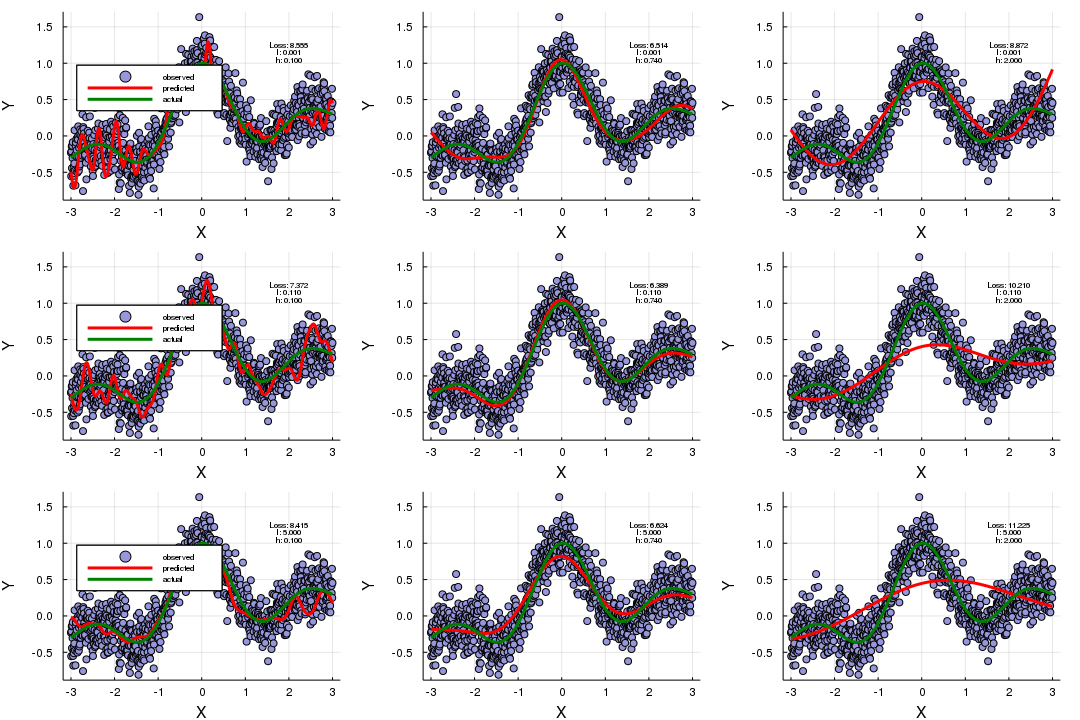
\includegraphics[clip, scale=0.4]{fitting.png}
    \caption{パラメータを変化させた結果}
    \label{fig:cv}
  \end{center}
\end{figure}
\section{宿題2}
Julia 1.0.0で実装した。
\begin{lstlisting}
using Plots


mutable struct SVMResult
    n::Int64
    epsilon::Float64
    h::Float64
    C::Float64
    theta::VecOrMat{Float64}
    x::VecOrMat{Float64}
    y::VecOrMat{Float64}
    k::Matrix{Float64}
    converged::Bool
end

function SVM(
    x::Matrix{T}, 
    y::VecOrMat{T}, 
    C::Float64, 
    h::Float64;
    epsilon::Float64=0.01, 
    maxiter::Int64=10000, 
    tol::Float64=1e-6) where T<:AbstractFloat

    n = Int(length(x) / 2)
    @assert n == length(y)
    xx = x[:, 1]
    xy = x[:, 2]
    xx2 = xx .^ 2
    xy2 = xy .^ 2
    k = exp.(
        -(
            (repeat(xx2, 1, n) + repeat(xx2', n, 1) - 2 .* (xx * xx')) + 
            (repeat(xy2, 1, n) + repeat(xy2', n, 1) - 2 .* (xy * xy'))
        ) ./ (2 * h^2)
    )
    theta = rand(n, 1)
    converged = false
    cnt = 1
    while !converged && cnt < maxiter
        delThetaj = ifelse.(
            ones(n, 1) - (k * theta) .* y .> 0,
            - y .* k,
            0
        )
        sum_delTheta = sum(delThetaj, dims=1)'
        new_theta = theta - epsilon .* (C .* sum_delTheta + 2 .* (k * theta))
        if sqrt(sum((theta - new_theta).^2)) > tol
            theta = new_theta
            cnt += 1
        else
            theta = new_theta
            converged = true
        end
    end
    SVMResult(n, epsilon, h, C, theta, x, y, k, converged)
end
    
n = 200
a = collect(range(0, stop=4 * pi, length=Int(n/2)))
u = append!(a .* cos.(a), (a .+ pi) .* cos.(a)) + rand(n, 1)
v = append!(a .* sin.(a), (a .+ pi) .* sin.(a)) + rand(n, 1)
x = [u v]
y = append!(reshape(ones(1, Int(n/2)), (100,)), reshape(-ones(1, Int(n/2)), (100,)))
    
svm = SVM(x, y, 0.1, 0.3)
m = 100
X = collect(range(-15, stop=15, length=m))
X2 = X .^ 2
U=exp.(-(repeat(u.^2,1,m)+repeat(X2',n,1)-2 .* (u*X'))/ (2 * svm.h^2))
V=exp.(-(repeat(v.^2,1,m)+repeat(X2',n,1)-2 .* (v*X'))/ (2 * svm.h^2))
p = contour(X, X, sign.(V' * (U .* repeat(svm.theta, 1, m))), 
    fill=true,
    fillcolor=:viridis,
    fillalpha=0.1,
    xlabel="X",
    ylabel="Y",
    xlims=(-15, 15),
    ylims=(-15, 15)
)
scatter!(p, u[1:100], v[1:100], y[1:100], color=:yellow, label="Class1", ticks=false)
scatter!(p, u[101:200], v[101:200], y[101:200], color=:red, label="Class2", ticks=false)
png("svm")
\end{lstlisting}
結果は、図\ref{fig:svm}のようになった。
\begin{figure}[h]
\begin{center}
\includegraphics[clip, scale=0.8]{svm.png}
\caption{SVMによる分類}
\label{fig:svm}
\end{center}
\end{figure}
\end{document}
